% Unofficial UofT Poster template.
% A fork of the UMich template https://www.overleaf.com/latex/templates/university-of-michigan-umich-poster-template/xpnqzzxwbjzc
% which is fork of the MSU template https://www.overleaf.com/latex/templates/an-unofficial-poster-template-for-michigan-state-university/wnymbgpxnnwd
% which is a fork of https://www.overleaf.com/latex/templates/an-unofficial-poster-template-for-new-york-university/krgqtqmzdqhg
% which is a fork of https://github.com/anishathalye/gemini
% also refer to https://github.com/k4rtik/uchicago-poster

\documentclass[final]{beamer}

% ====================
% Packages
% ====================

\usepackage[T1]{fontenc}
 \usepackage[utf8]{luainputenc}
\usepackage{lmodern}
\usepackage[size=custom, width=122,height=91, scale=1.2]{beamerposter}
\usetheme{gemini}
\usecolortheme{uoft}
\usepackage{graphicx}
\usepackage{booktabs}
\usepackage{tikz}
\usepackage{pgfplots}
\pgfplotsset{compat=1.14}
\usepackage{anyfontsize}

\usepackage{tikz}
\usetikzlibrary{decorations.pathreplacing}

% ====================
% Lengths
% ====================

% If you have N columns, choose \sepwidth and \colwidth such that
% (N+1)*\sepwidth + N*\colwidth = \paperwidth
\newlength{\sepwidth}
\newlength{\colwidth}
\setlength{\sepwidth}{0.025\paperwidth}
\setlength{\colwidth}{0.3\paperwidth}

\newcommand{\separatorcolumn}{\begin{column}{\sepwidth}\end{column}}

% ====================
% Title
% ====================

\title{Neural Style Transfer:\\ Fundamental Theory and Architecture}

\author{Jingwen (Steven) Shi}

\institute[shortinst]{University of Toronto}

% ====================
% Footer (optional)
% ====================

\footercontent{
  \href{https://github.com/jingwenshi-dev/NST-Poster}{Github: https://github.com/jingwenshi-dev/NST-Poster} \hfill
CSC490 2023 Fall \hfill
  \href{mailto:jingwensteven.shi@mail.utoronto.ca}{jingwensteven.shi@mail.utoronto.ca}}
% (can be left out to remove footer)

% ====================
% Logo (optional)
% ====================

% use this to include logos on the left and/or right side of the header:
% Left: institution
 \logoright{
\includegraphics[height=8cm]{logos/logo.png}}
% Right: funding agencies and other affilations 
%\logoright{\includegraphics[height=7cm]{logos/NSF.eps}}
% ====================
% Body
% ====================

\begin{document}
\begin{frame}[t]
\begin{columns}[t]
\separatorcolumn

\begin{column}{\colwidth}

    \begin{block}{Abstract}
    
        This poster aims to provide a comprehensive overview of key concepts in neural style transfer including architecture, loss functions, transfer learning, target detaching, and layer choices.
    
    \end{block}

    \begin{block}{Architecture}
    
        Based on the VGG-19 pre-trained model with style loss and content loss layers inserted:

        \begin{figure}
          \centering
            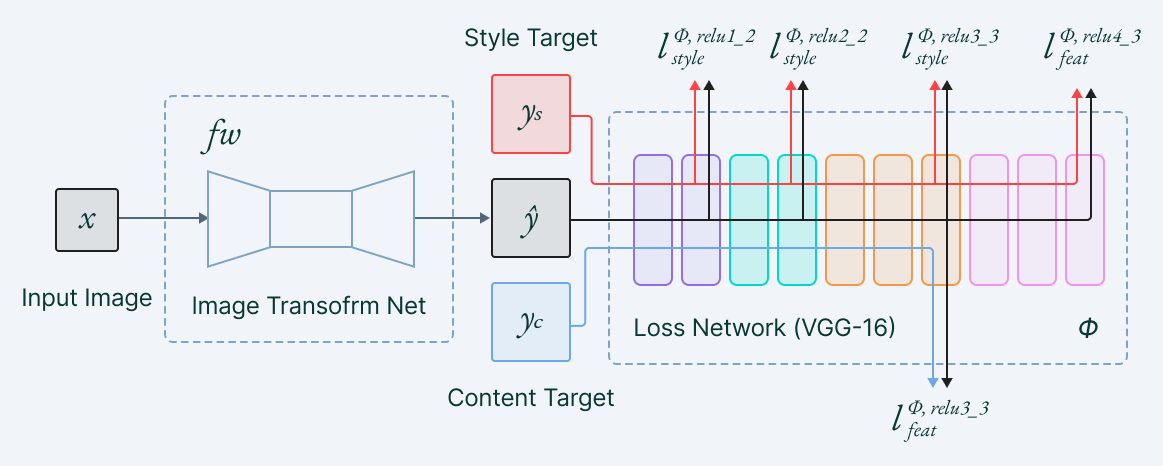
\includegraphics[width=1\textwidth]{figures/NST Architecture.png}
        
            \caption{Neural Style Transfer Architecture (source: V7 Labs)}
        \end{figure}
        
        The model does not include all the layers of VGG-19. In fact, the model got cut off and abandoned all the layers after the last loss layer was inserted for several reasons:
        \begin{itemize}
            \item \textbf{Focus on Style Features:\\}
            Neural style transfer aims to merge the content of an image with the style of another. By cutting off the model after the last loss layer, the model can focus on the style feature better and the rest of the VGG-19 layers are simply not helpful.
            \item \textbf{Computation Efficiency:\\}
            VGG-19 is a type of CNN model, the more layers a model has, the more computing-intensive it is. By cutting off the model, the layers are not necessarily for capturing content and style will not be computed.
        \end{itemize}

        \begin{figure}
          \centering
            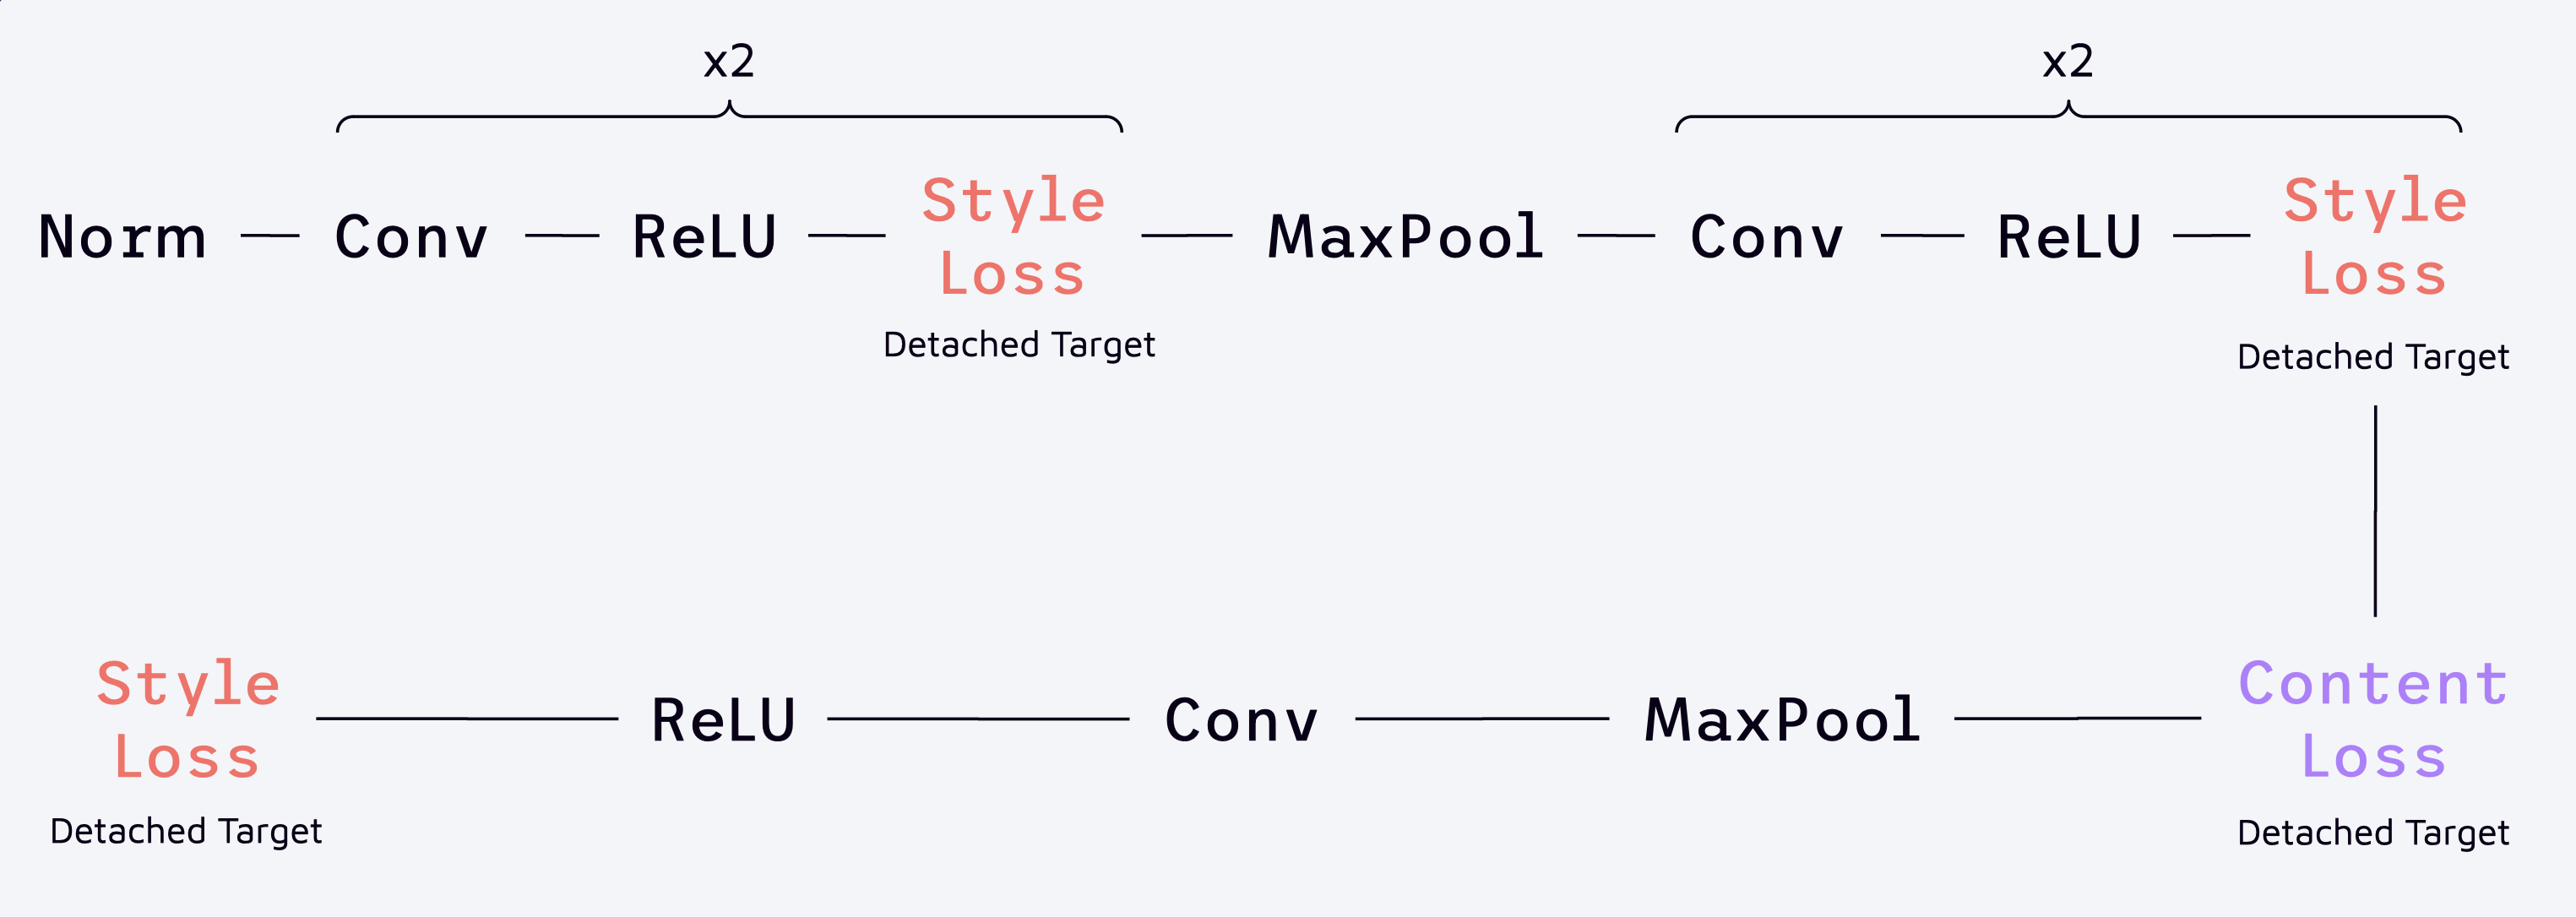
\includegraphics[width=1\textwidth]{figures/NST Flowchart.png}
        
            \caption{Neural Style Transfer Flowchart}
        \end{figure}
    
    \end{block}

\end{column}

\separatorcolumn

\begin{column}{\colwidth}

  \begin{block}{Total Loss}

    The complete loss is the sum of the content and style loss since the goal is to minimize the joint losses on the generated image.

    $$
    \mathcal{L}_{total}(p, a, x) = \alpha\mathcal{L}_{content}(p, x) + \beta\mathcal{L}_{style}(a, x)
    $$
    where:
    \begin{itemize}
        \item $\alpha$ and $\beta$ are weighting factors that determine the relative importance of the content and style.
        \item p, a, x are the content, style, and input images.
    \end{itemize}

  \end{block}

  \begin{block}{Content Loss}

    Each content loss is the mean square error (MSE) between the feature representation of content and the input image. It measures the difference between the generated image and the content image.

    $$\mathcal{L}_{content}(p, x, l) = \frac{1}{n} \sum_{i, j}(F^l_{i, j}(x) - F^l_{i, j}(p))^2$$
    where:
    \begin{itemize}
        \item $p$ is the content image.
        \item $x$ is the input image.
        \item $F^l_{i, j}$ is the feature map at layer l.
    \end{itemize}

  \end{block}

  \begin{block}{Style Loss}

    Style loss uses the same methodology as content loss to calculate the distance between the feature maps.
    
    $$\mathcal{L}_{style}(a, x, l) = \frac{1}{4 N^2_l M^2_l} \sum (G^l(x) - G^l(a))^2 $$
    where:
    \begin{itemize}
        \item $a$ is the style image.
        \item $x$ is the input image.
        \item $\frac{1}{4 N^2_l M^2_l}$ is the normalization factor.
            \begin{itemize}
                \vskip1ex
                \item N is the number of feature maps.
                \item M is the size of each feature map.
                \item 4 scales down the values to make the products of multiplications manageable.
                \vskip1ex
            \end{itemize}
        \item $G^l = F \cdot F^T$ is the Gram matrix of the feature map at layer $l$
        \item $N_l$ is the number of feature maps at layer $l$.
        \item $M_l$ is the size of each feature map at layer $l$.
    \end{itemize}

    \heading{Role of Gram Matrix}
    The Gram matrix is the product of a feature map with its transpose. It captures the coloration between feature maps which represents the style of the image.

  \end{block}

\end{column}

\separatorcolumn

\begin{column}{\colwidth}

  \begin{alertblock}{Why not Covariance Matrix}

    In the formula below, it is clear that the only major difference between the Gram and covariance matrices is that the Gram matrix does not subtract from the sample mean.
    
    $$Cov = \frac{1}{N-1} (F-\bar{F})\cdot(F-\bar{F})^T$$

    This ignores the spatial arrangement of the features and is ideal for capturing the overall style of the textures:

    \begin{enumerate}
        \item In the covariance matrix, the mean of each feature is subtracted from the feature values which center the data with respect to 0.
        \item In image processing, these features may related to pixel intensities (i.e. RGB values) and centers data around the mean will capture the intensity of one feature related to the presence of another.
        \item Gram matrix does not subtract from the mean which only focuses on the overall frequency of feature co-occurrences.
    \end{enumerate}

    The elements like brushstrokes and colour palettes are parts of the style that should not depend on the positioning of objects. Therefore, the ability that the Gram matrix can abstract away from these spatial relationships and only focus on the overall presence of the feature maps, is exactly what we need.

  \end{alertblock}

  \begin{exampleblock}{Choice of Layers}

    \textbf{Content Layers: \{ReLU 10\}}\\
    
    \textbf{Style Layers: \{ReLU 1, ReLU 3, ReLU 5, ReLU 9, ReLU 13\}}

    \heading{Properties of Layer}
    \begin{enumerate}
        \item The lower the layer, the better it can capture the details and patterns of an image.
        \item The higher the layer, the better it can capture the overall abstraction of an image.
    \end{enumerate}

    \heading{Why ReLU 1, 3, 5, 9, 13?}
    Since the input is a copy of the content image, lower style layers can quickly merge the style patterns to the input image.

    \heading{Why ReLU 10?}
    A middle content layer can effectively preserve the input's content. If a lower content layer is used, the output will closely resemble pixel-level copies of the content. However, given that the input is already a replication of the content image, there's no necessity to employ a lower content layer, as it might overshadow the style.

  \end{exampleblock}

  \begin{block}{References}

    \nocite{*}
    \footnotesize{\bibliographystyle{plain}\bibliography{poster}}

  \end{block}

\end{column}

\separatorcolumn
\end{columns}
\end{frame}

\end{document}
